%%%%%%%%%%%%%%%%%%%%%%%%%%%%%%%%%%%%%%%%%
% Beamer Presentation
% LaTeX Template
% Version 1.0 (10/11/12)
%
% This template has been downloaded from:
% http://www.LaTeXTemplates.com
%
% License:
% CC BY-NC-SA 3.0 (http://creativecommons.org/licenses/by-nc-sa/3.0/)
%
%%%%%%%%%%%%%%%%%%%%%%%%%%%%%%%%%%%%%%%%%

%----------------------------------------------------------------------------------------
%	PACKAGES AND THEMES
%----------------------------------------------------------------------------------------

\documentclass{beamer}

\mode<presentation> {

% The Beamer class comes with a number of default slide themes
% which change the colors and layouts of slides. Below this is a list
% of all the themes, uncomment each in turn to see what they look like.

\usetheme{default}
%\usetheme{AnnArbor}
%\usetheme{Antibes}
%\usetheme{Bergen}
%\usetheme{Berkeley}
%\usetheme{Berlin}
%\usetheme{Boadilla}
%\usetheme{CambridgeUS}
%\usetheme{Copenhagen}
%\usetheme{Darmstadt}
%\usetheme{Dresden}
%\usetheme{Frankfurt}
%\usetheme{Goettingen}
%\usetheme{Hannover}
%\usetheme{Ilmenau}
%\usetheme{JuanLesPins}
%\usetheme{Luebeck}
%\usetheme{Madrid}
%\usetheme{Malmoe}
%\usetheme{Marburg}
%\usetheme{Montpellier}
%\usetheme{PaloAlto}
%\usetheme{Pittsburgh}
%\usetheme{Rochester}
%\usetheme{Singapore}
%\usetheme{Szeged}
%\usetheme{Warsaw}

% As well as themes, the Beamer class has a number of color themes
% for any slide theme. Uncomment each of these in turn to see how it
% changes the colors of your current slide theme.

%\usecolortheme{albatross}
%\usecolortheme{beaver}
%\usecolortheme{beetle}
%\usecolortheme{crane}
%\usecolortheme{dolphin}
%\usecolortheme{dove}
%\usecolortheme{fly}
%\usecolortheme{lily}
%\usecolortheme{orchid}
%\usecolortheme{rose}
%\usecolortheme{seagull}
%\usecolortheme{seahorse}
%\usecolortheme{whale}
%\usecolortheme{wolverine}

%\setbeamertemplate{footline} % To remove the footer line in all slides uncomment this line
\setbeamertemplate{footline}[page number] % To replace the footer line in all slides with a simple slide count uncomment this line

\setbeamertemplate{navigation symbols}{} % To remove the navigation symbols from the bottom of all slides uncomment this line
}
\newenvironment{changemargin}[2]{%
\begin{list}{}{%
\setlength{\topsep}{0pt}%
\setlength{\leftmargin}{#1}%
\setlength{\rightmargin}{#2}%
\setlength{\listparindent}{\parindent}%
\setlength{\itemindent}{\parindent}%
\setlength{\parsep}{\parskip}%
}%
\item[]}{\end{list}}
%\usepackage[greek,german]{babel}
\usepackage{graphicx} % Allows including images
\usepackage{booktabs} % Allows the use of \toprule, \midrule and \bottomrule in tables
\usepackage{amsmath}
\usepackage{slashed}
\usepackage{color}
\usepackage{rotating}
%----------------------------------------------------------------------------------------
%	TITLE PAGE
%----------------------------------------------------------------------------------------

\title{LFV lephad analysis status report} % The short title appears at the bottom of every slide, the full title is only on the title page

\author{\underline{Author} \and Author} % Your name

\author{A.~Pathak, S.~Banerjee, P.N.~Dang and D.~Biswas}


\institute{\begin{minipage}{0.5\textwidth}\centering
\includegraphics[scale=0.1]{/afs/cern.ch/user/s/swaban/public/university-of-louisville-logo.png}
\end{minipage}}
\date{{LFV lephad meeting}\\\today\\} % Date, can be changed to a custom date


\begin{document}

\begin{frame}
\titlepage % Print the title page as the first slide
\end{frame}
%-----------------------------------------------
\begin{frame}
\frametitle{Postfit plots for H$\rightarrow \mu\tau_{had}$ for combined SR'+VBF}
\begin{normalsize}
Default bin(top) and Leplep bin(bottom)
\vspace*{0.5cm}
\includegraphics[width=.25\textwidth,height=.30\textheight,type=pdf,ext=.png,read=.png]{/afs/cern.ch/user/a/atpathak/afswork/public/Pixel/LFV_Plots/postfit/mtau_comb_sr_vbf_new/MColl_mtau_sr1_vbf_signal_}
\includegraphics[width=.25\textwidth,height=.30\textheight,type=pdf,ext=.png,read=.png]{/afs/cern.ch/user/a/atpathak/afswork/public/Pixel/LFV_Plots/postfit/mtau_comb_sr_vbf_new/MColl_mtau_sr2_vbf_signal_}
\includegraphics[width=.25\textwidth,height=.30\textheight,type=pdf,ext=.png,read=.png]{/afs/cern.ch/user/a/atpathak/afswork/public/Pixel/LFV_Plots/postfit/mtau_comb_sr_vbf_new/MColl_mtau_sr3_vbf_signal_}
\includegraphics[width=.25\textwidth,height=.30\textheight,type=pdf,ext=.png,read=.png]{/afs/cern.ch/user/a/atpathak/afswork/public/Pixel/LFV_Plots/postfit/mtau_comb_sr_vbf_new/MColl_mtau_cba_vbf_signal_}\\
\includegraphics[width=.25\textwidth,height=.30\textheight,type=pdf,ext=.png,read=.png]{/afs/cern.ch/user/a/atpathak/afswork/public/Pixel/LFV_Plots/postfit/mtau_comb_sr_vbf_llbin/MColl_mtau_sr1_vbf_signal_}
\includegraphics[width=.25\textwidth,height=.30\textheight,type=pdf,ext=.png,read=.png]{/afs/cern.ch/user/a/atpathak/afswork/public/Pixel/LFV_Plots/postfit/mtau_comb_sr_vbf_llbin/MColl_mtau_sr2_vbf_signal_}
\includegraphics[width=.25\textwidth,height=.30\textheight,type=pdf,ext=.png,read=.png]{/afs/cern.ch/user/a/atpathak/afswork/public/Pixel/LFV_Plots/postfit/mtau_comb_sr_vbf_llbin/MColl_mtau_sr3_vbf_signal_}
\includegraphics[width=.25\textwidth,height=.30\textheight,type=pdf,ext=.png,read=.png]{/afs/cern.ch/user/a/atpathak/afswork/public/Pixel/LFV_Plots/postfit/mtau_comb_sr_vbf_llbin/MColl_mtau_cba_vbf_signal_}\\
\hspace{0.5in}SR1 
\hspace{0.75in}SR2
\hspace{0.75in}SR3
\hspace{0.75in}VBF
\end{normalsize}
\end{frame}
%-----------------------------------------------
\begin{frame}
\frametitle{Postfit plots for H$\rightarrow e\tau_{had}$ for combined SR'+VBF}
\begin{normalsize}
Default bin(top) and Leplep bin(bottom)
\vspace*{0.5cm}
\includegraphics[width=.25\textwidth,height=.30\textheight,type=pdf,ext=.png,read=.png]{/afs/cern.ch/user/a/atpathak/afswork/public/Pixel/LFV_Plots/postfit/etau_comb_sr_vbf/MColl_etau_sr1_vbf_signal_}
\includegraphics[width=.25\textwidth,height=.30\textheight,type=pdf,ext=.png,read=.png]{/afs/cern.ch/user/a/atpathak/afswork/public/Pixel/LFV_Plots/postfit/etau_comb_sr_vbf/MColl_etau_sr2_vbf_signal_}
\includegraphics[width=.25\textwidth,height=.30\textheight,type=pdf,ext=.png,read=.png]{/afs/cern.ch/user/a/atpathak/afswork/public/Pixel/LFV_Plots/postfit/etau_comb_sr_vbf/MColl_etau_sr3_vbf_signal_}
\includegraphics[width=.25\textwidth,height=.30\textheight,type=pdf,ext=.png,read=.png]{/afs/cern.ch/user/a/atpathak/afswork/public/Pixel/LFV_Plots/postfit/etau_comb_sr_vbf/MColl_etau_cba_vbf_signal_}\\

\includegraphics[width=.25\textwidth,height=.30\textheight,type=pdf,ext=.png,read=.png]{/afs/cern.ch/user/a/atpathak/afswork/public/Pixel/LFV_Plots/postfit/etau_comb_sr_vbf_llbin/MColl_etau_sr1_vbf_signal_}
\includegraphics[width=.25\textwidth,height=.30\textheight,type=pdf,ext=.png,read=.png]{/afs/cern.ch/user/a/atpathak/afswork/public/Pixel/LFV_Plots/postfit/etau_comb_sr_vbf_llbin/MColl_etau_sr2_vbf_signal_}
\includegraphics[width=.25\textwidth,height=.30\textheight,type=pdf,ext=.png,read=.png]{/afs/cern.ch/user/a/atpathak/afswork/public/Pixel/LFV_Plots/postfit/etau_comb_sr_vbf_llbin/MColl_etau_sr3_vbf_signal_}
\includegraphics[width=.25\textwidth,height=.30\textheight,type=pdf,ext=.png,read=.png]{/afs/cern.ch/user/a/atpathak/afswork/public/Pixel/LFV_Plots/postfit/etau_comb_sr_vbf_llbin/MColl_etau_cba_vbf_signal_}\\
\hspace{0.5in}SR1 
\hspace{0.75in}SR2
\hspace{0.75in}SR3
\hspace{0.75in}VBF
\end{normalsize}
\end{frame}
%-----------------------------------------------
\end{document}
%-----------------------------------------------
\begin{frame}
\frametitle{NP Ranking for combined $\mu\tau_{had}$ for no ASL}
\begin{normalsize}
\hspace{1.2in}Default bin 
\hspace{1.5in}Leplep bin
\vspace*{0.2cm}
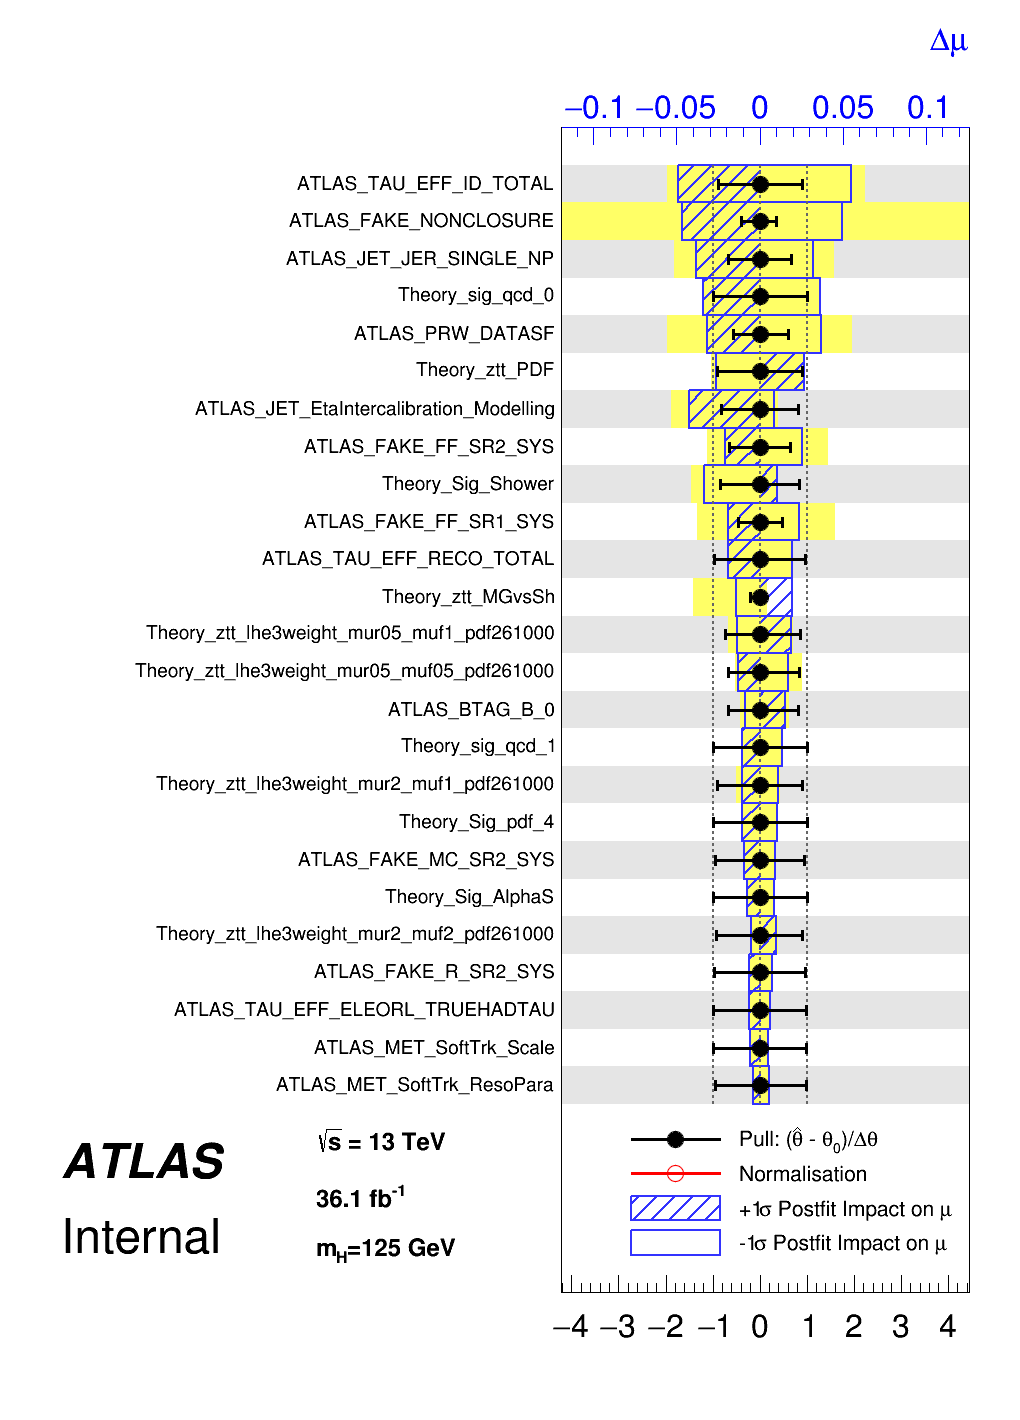
\includegraphics[width=.50\textwidth,height=.70\textheight,type=pdf,ext=.pdf,read=.pdf]{/afs/cern.ch/user/a/atpathak/afswork/public/WSMaker/pdf-files/version/mtau_comb_sr_vbf_noAgg_pulls_125}
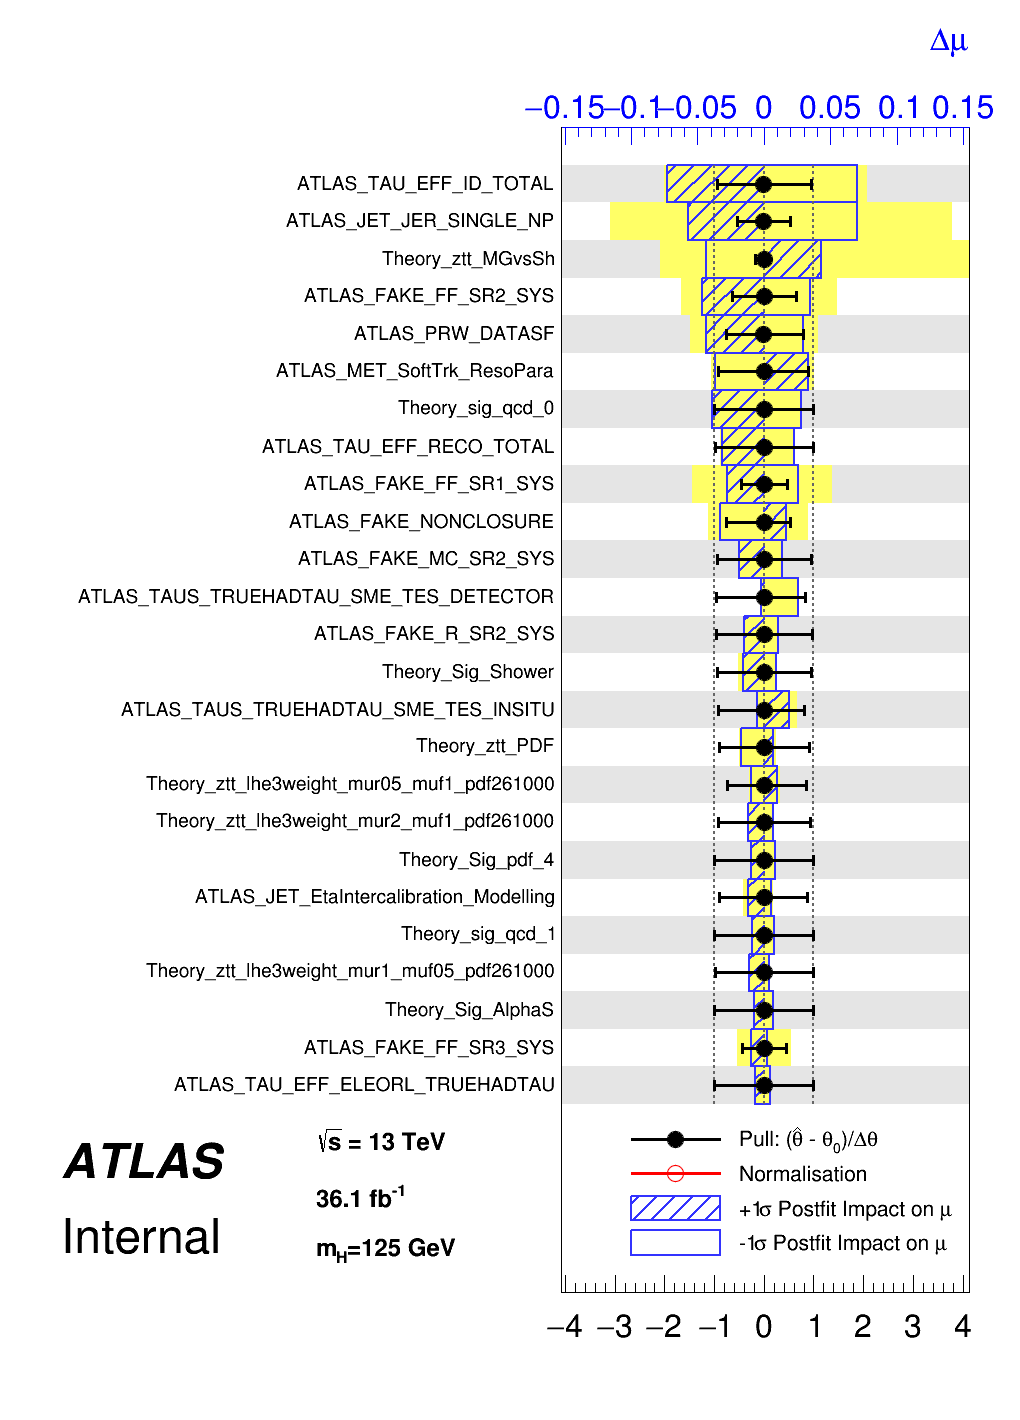
\includegraphics[width=.50\textwidth,height=.70\textheight,type=pdf,ext=.pdf,read=.pdf]{/afs/cern.ch/user/a/atpathak/afswork/public/WSMaker/pdf-files/version/mtau_comb_sr_vbf_llbin_noAgg_pulls_125}
\end{normalsize}
\end{frame}
%-----------------------------------------------
\begin{frame}
\frametitle{NP Ranking for combined $e\tau_{had}$ for with ASL}
\begin{normalsize}
\hspace{1.2in}Default bin 
\hspace{1.5in}Leplep bin
\vspace*{0.2cm}
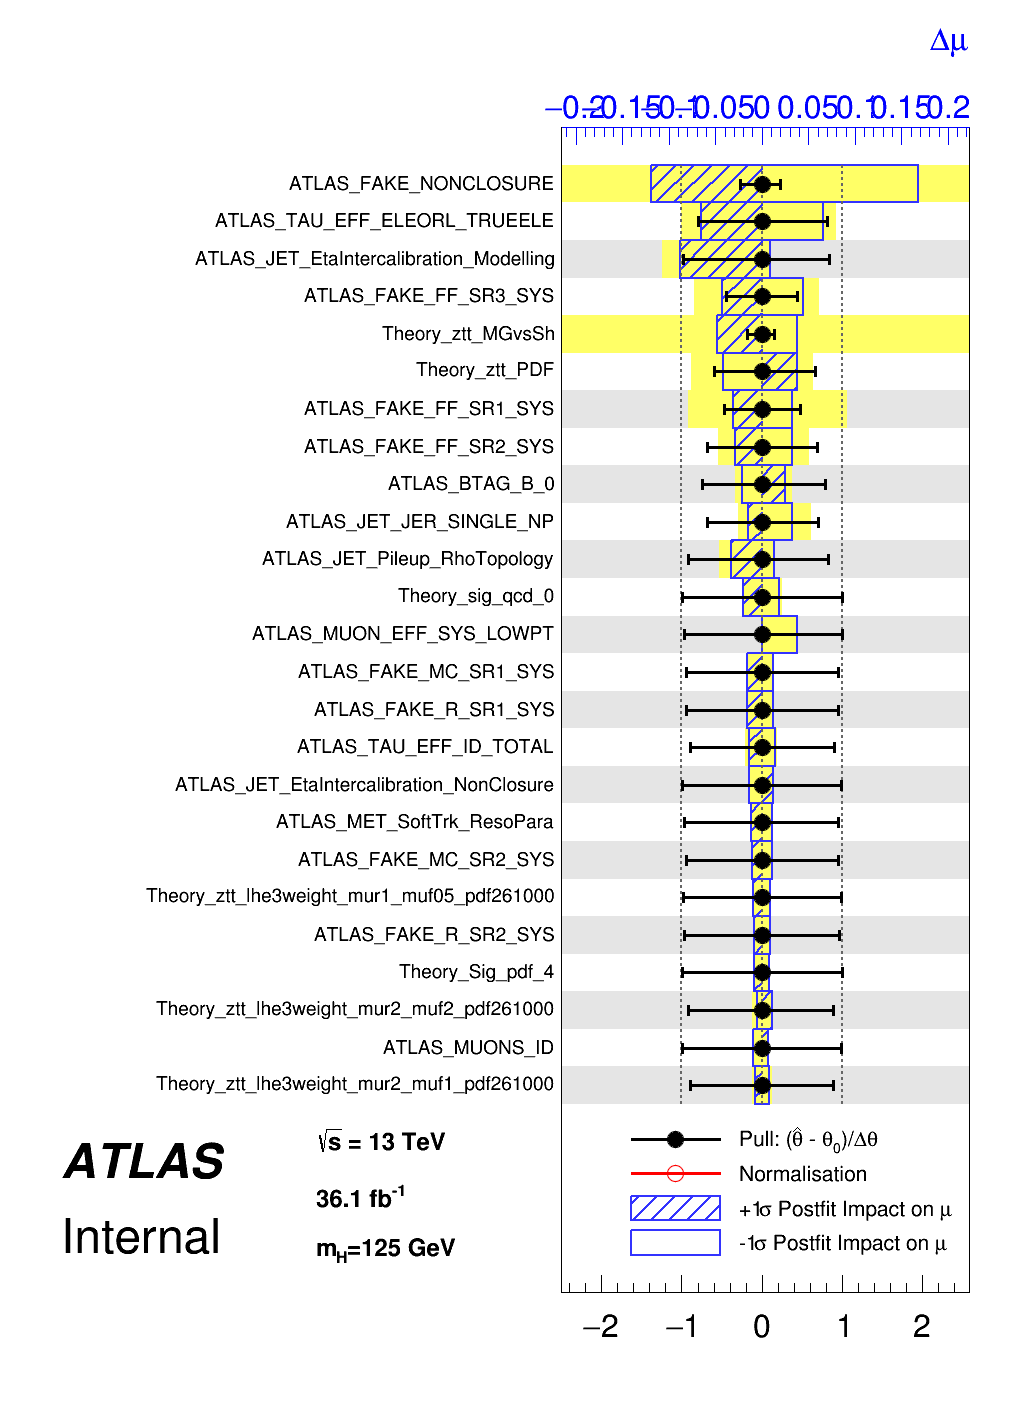
\includegraphics[width=.50\textwidth,height=.70\textheight,type=pdf,ext=.pdf,read=.pdf]{/afs/cern.ch/user/a/atpathak/afswork/public/WSMaker/pdf-files/version/etau_comb_sr_vbf_pulls_125}
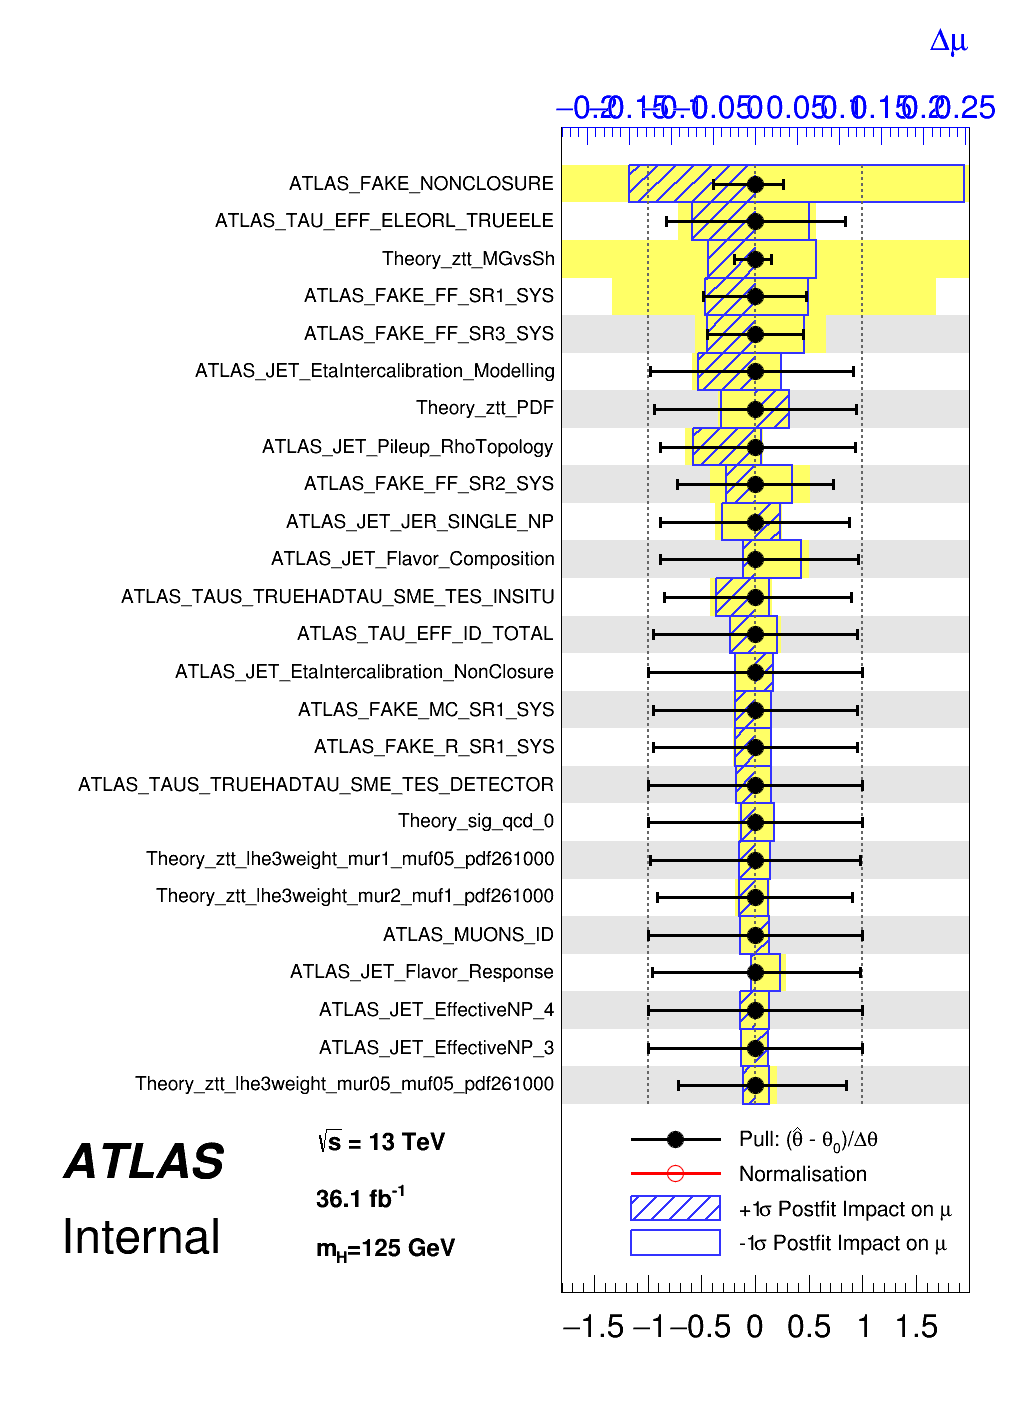
\includegraphics[width=.50\textwidth,height=.70\textheight,type=pdf,ext=.pdf,read=.pdf]{/afs/cern.ch/user/a/atpathak/afswork/public/WSMaker/pdf-files/version/etau_comb_sr_vbf_llbin_pulls_125}
\end{normalsize}
\end{frame}
%-----------------------------------------------
\begin{frame}
\frametitle{NP Ranking for combined $e\tau_{had}$ for no ASL}
\begin{normalsize}
\hspace{1.2in}Default bin 
\hspace{1.5in}Leplep bin
\vspace*{0.2cm}
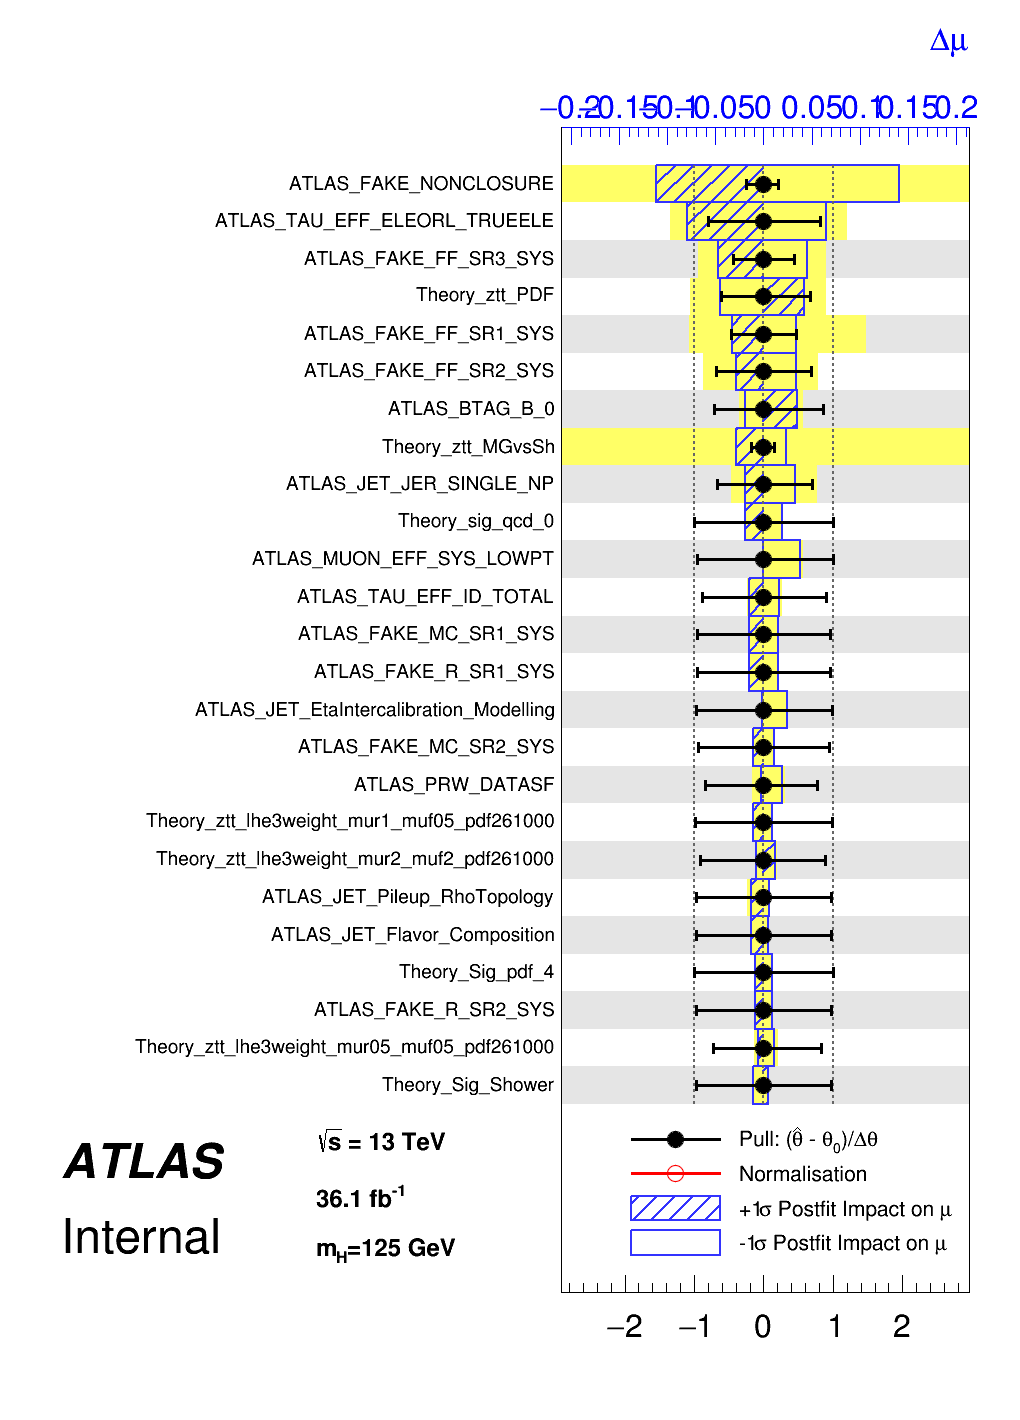
\includegraphics[width=.50\textwidth,height=.70\textheight,type=pdf,ext=.pdf,read=.pdf]{/afs/cern.ch/user/a/atpathak/afswork/public/WSMaker/pdf-files/version/etau_comb_sr_vbf_noAgg_pulls_125}
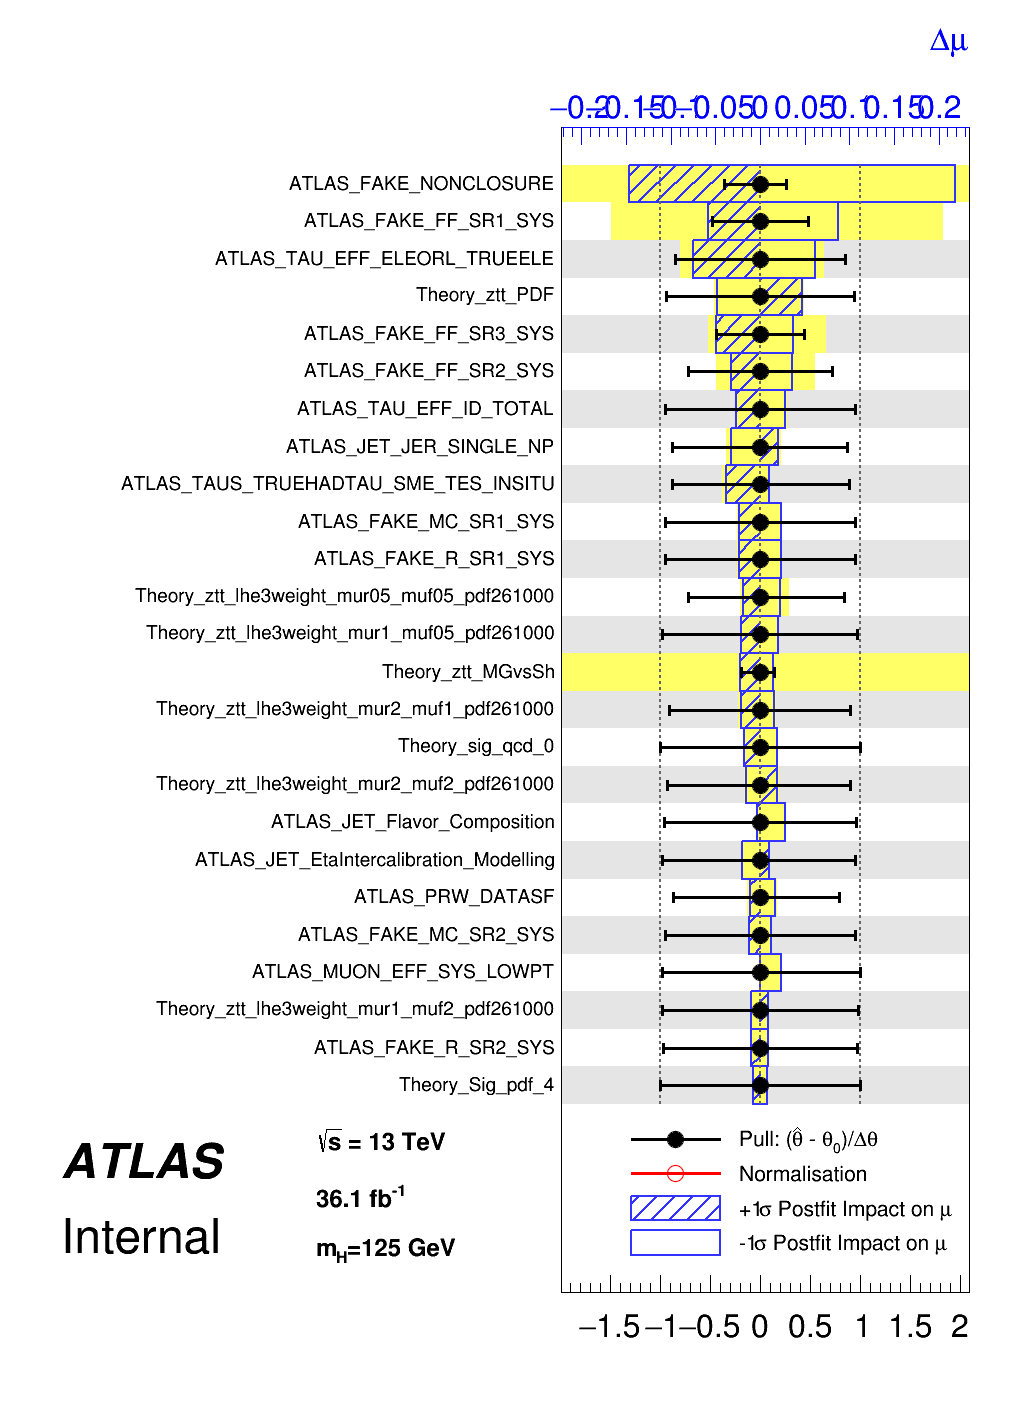
\includegraphics[width=.50\textwidth,height=.70\textheight,type=pdf,ext=.pdf,read=.pdf]{/afs/cern.ch/user/a/atpathak/afswork/public/WSMaker/pdf-files/version/etau_comb_sr_vbf_llbin_noAgg_pulls_125}
\end{normalsize}
\end{frame}
